\section{Investigation of Genome Properties}
\label{sec:properties}
The process of running a task-solving experiments such as in the preceding sections is quite opaque.
The experiment is configured by human, but after it is started the system runs itself with no human input,
and the human observer can only wait and hope a useful result emerges at the end.

In order to gain a better understanding of the process,
an experiment was designed with the goal of investigating various properties of the population and their development over time,
rather than to solve a specific task.
This involves storing every single individual from the whole run, then analyzing them quantitatively afterwards.

CA-NEAT can be studied from multiple "angles": as a GA experiment there are properties such as fitness that can be studied,
as a CA experiment there is for example the $\lambda$ parameterization,
and as a graph-based encoding properties such as the number of nodes can be investigated.
Inspecting these, individually and trying to see correlation, should help with understand the system better,
and selecting better configurations for future experiments.

There are also multiple different mechanisms of the algorithm that can enabled or disabled by configuration.
Running multiple GA runs with different combinations of mechanisms enabled should give some indication about the effects of the mechanism.

\subsection{Experiment Design}
The "Swiss" morphogenesis task is used as the basis for this experiment,
since previous experiments with this problem showed it to be consistently solvable by CA-NEAT, but not trivially simple.
The fitness evaluation for morphogenesis problems is also very fast compared to other problems, making it possible to run tests with large populations in a reasonable amount of time.
The CA for this problem has $K=2$ cell states and the neighborhood shape "Von Neumann" ($N=5$) was used.
An initial population of size $P=1000$ was created, with $N$ input nodes, $K$ output nodes and no initial hidden nodes.
This same population was then used as the initial population for five independent "scenarios" of $G=100$ generations, with different mechanisms of NEAT in use.
Table \ref{tbl:NEAT_incremental} shows which mechanisms are in use in which scenario.
From top to bottom, the table can be read as gradually enabling mechanisms, until arriving at the full algorithm, as used in other experiments.

\begin{table}
    \centering
    \caption{Mechanisms enabled in different scenarios}
    \begin{tabular}{c|ccccc}
    Scenario & Mutation & Crossover & Selection pressure & Speciation & Elitism \\ \hline
    A   & \checkmark        & ~         & ~                  & ~          & ~       \\
    B   & \checkmark        & \checkmark         & ~                  & ~          & ~       \\
    C   & \checkmark        & \checkmark         & \checkmark                  & ~          & ~       \\
    D   & \checkmark        & \checkmark         & \checkmark                  & \checkmark          & ~       \\
    E   & \checkmark        & \checkmark         & \checkmark                  & \checkmark          & \checkmark       \\
    \end{tabular}
    \label{tbl:NEAT_incremental}
\end{table}

\begin{description}
\item[Scenario A] ~\\
Scenario A is different from the rest, since it is not a GA run, but more of a random walk in the search space using the mutation mechanism from the GA.
The individuals present in the initial population are mutated once per generation,
and the mutated versions are recorded as the next "generation".
With no crossover and no selection pressure, the individuals will be completely independent from each other throughout the entire run.
\item[Scenario B] ~\\
Scenario B uses NEAT, however the selection mechanism is completely randomized, so there is no selection pressure towards the goal of accomplishing the morphogenesis task.
\item[Scenario C] ~\\
Scenario C has selection pressure appropriate for the morphogenesis task, but does not use the speciation mechanism of NEAT.
\item[Scenario D] ~\\
Scenario D uses NEAT with selection pressure like C does, but also uses the speciation mechanism.
\item[Scenario E] ~\\
Scenario E uses all mechanisms of NEAT, including a per-species elitism degree of $E=1$.
\end{description}

Unlike the problem-solving experiments, this experiment does not involve multiple trials of the same configurations.
The reasoning is that this would mean we would be studying averages of averages in the following figures,
and some relationships between properties could be hidden by this.
We therefore should not draw any strong conclusions from the observations, but use it to find hypotheses that can be more rigorously investigated later.

\subsection{Fitness}
\begin{figure}
\centering
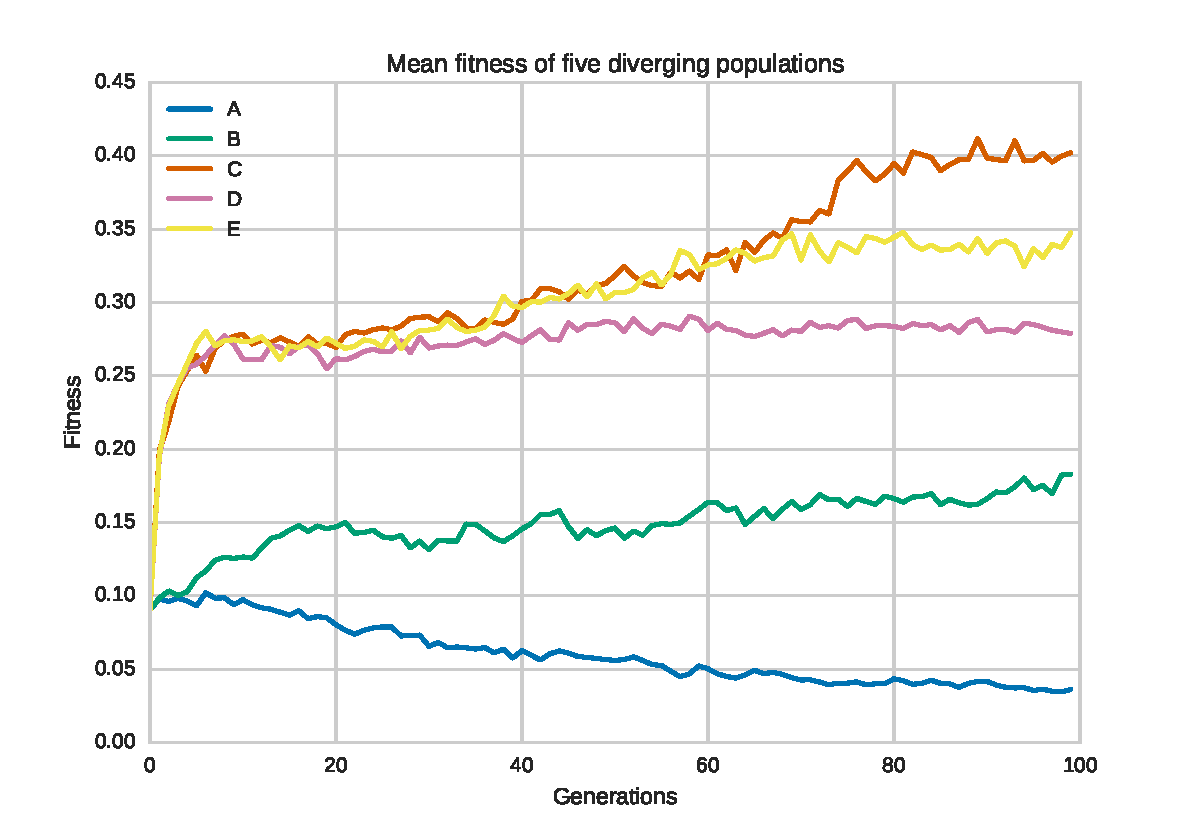
\includegraphics[width=\columnwidth]{fig/fitnesses}
\caption{The development over time of the mean fitness of the populations}
\label{fig:f_over_t}
\end{figure}

\begin{figure}
\centering
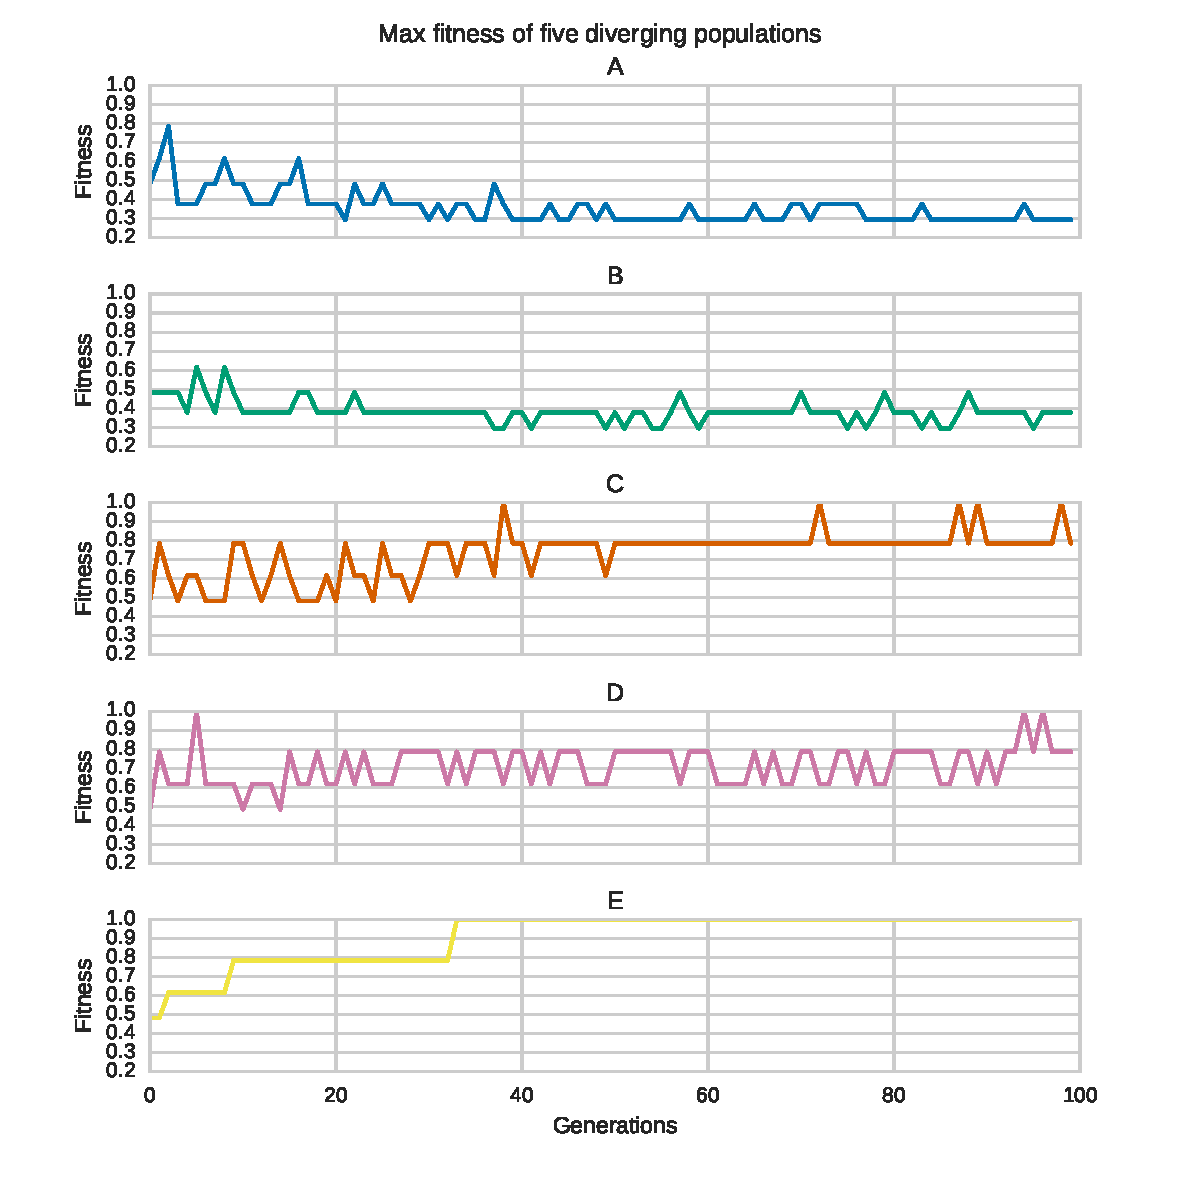
\includegraphics[width=\columnwidth]{fig/fitness_max}
\caption{The development over time of the max fitness of the populations}
\label{fig:max_fitness}
\end{figure}

When working with genetic algorithms, the most obvious property of a population to study is perhaps the average fitness over time.
Figure \ref{fig:f_over_t} shows the mean fitness development across the whole population for each of the five scenarios.
As one would expect, scenario A and B do not show any considerable improvement over time.
A declines steadily, while B has a slight, but not very significant increase.
Among C, D and E, which have selection pressure, there is a sharp increase in the first 10 generations.
D then flattens out for the remaining time, while C and E improves some more, at a slower rate.

Averaging hides one important aspect of the fitness distribution, namely the maximum value, which indicates "success" when it reaches $1.0$.
Looking at the maximum fitness development over time in Figure \ref{fig:max_fitness},
both A and B appears to decline over time, but B less so than A.
C and D act similar in that they hover around the upper half of the scale, sometimes finding a $1.0$ score, but are unable to stay stable there.
Whereas E, with the elitism mechanism is able to stay at $1.0$ once it finds it.
D finds a perfect solution quite early, but this seems likely to be a "fluke", since it losses it again and takes a long time to find another.
This is consistent with the results of the Swiss morphogenesis in Section \ref{sec:prev_work}, where in 100 independent trials, a few of them chanced upon an early solution.

The fact that the C average fitness overtakes both the D and E averages can hypothetically be explained by the difference the speciation mechanism makes.
In scenario C, the search can only optimize for fitness, so when it finds a good candidate it will make a large number of children for that candidate.
Scenarios D and E can optimize for diversity as well, searching in multiple directions.
When a good candidate is found in a species, its children will dominate only in that species,
while the other species continue their search unaffected.
Another possible factor is the stagnation check which is also part of the speciation mechanism.
This eliminates species that haven't improved average fitness in 15 generations.
If a species has "peaked", then it will be eliminated eventually, even if it's average fitness is above the population average.
In the task-solving experiments, the algorithm is stopped when a "perfect" solution is found, but in this experiment it is allowed to continue, so this effect can happen.

\subsection{Speciation}
\begin{figure}
\centering
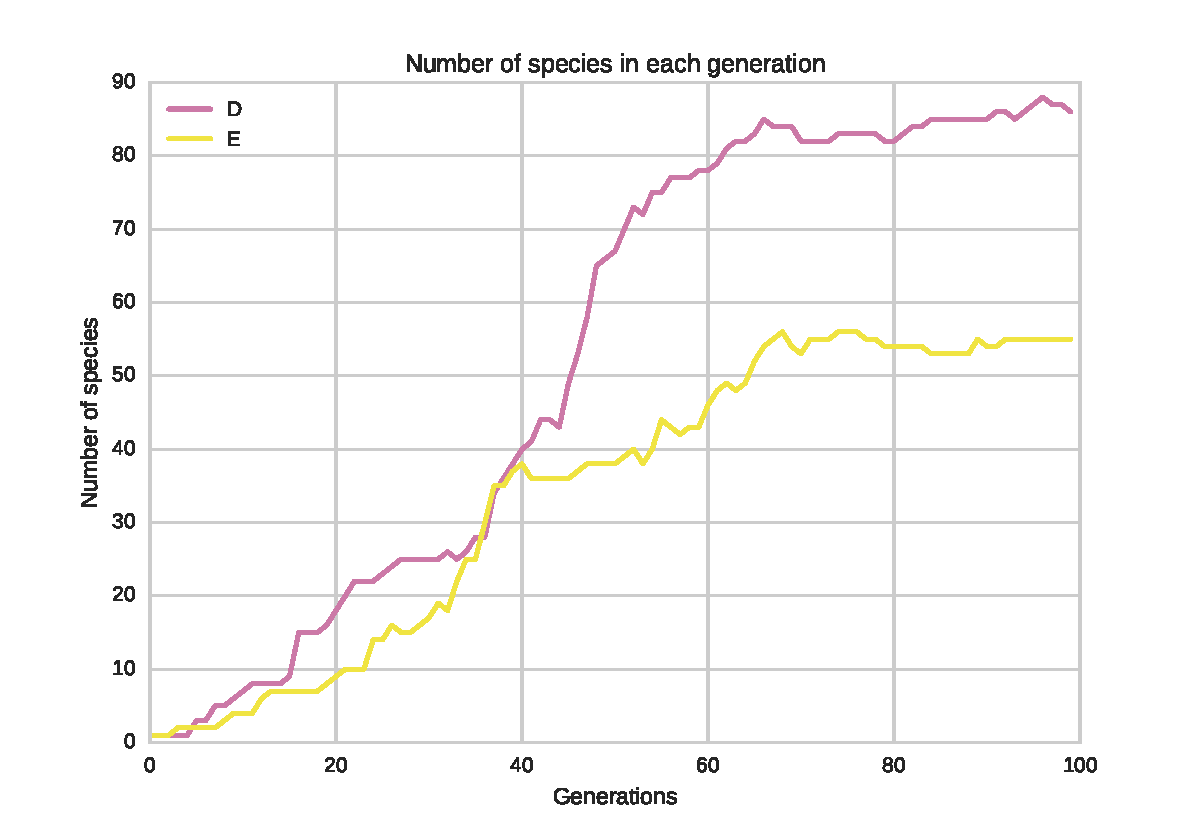
\includegraphics[width=\columnwidth]{fig/species}
\caption{The number of species in scenarios D and E over time}
\label{fig:species}
\end{figure}

\begin{figure}
\centering
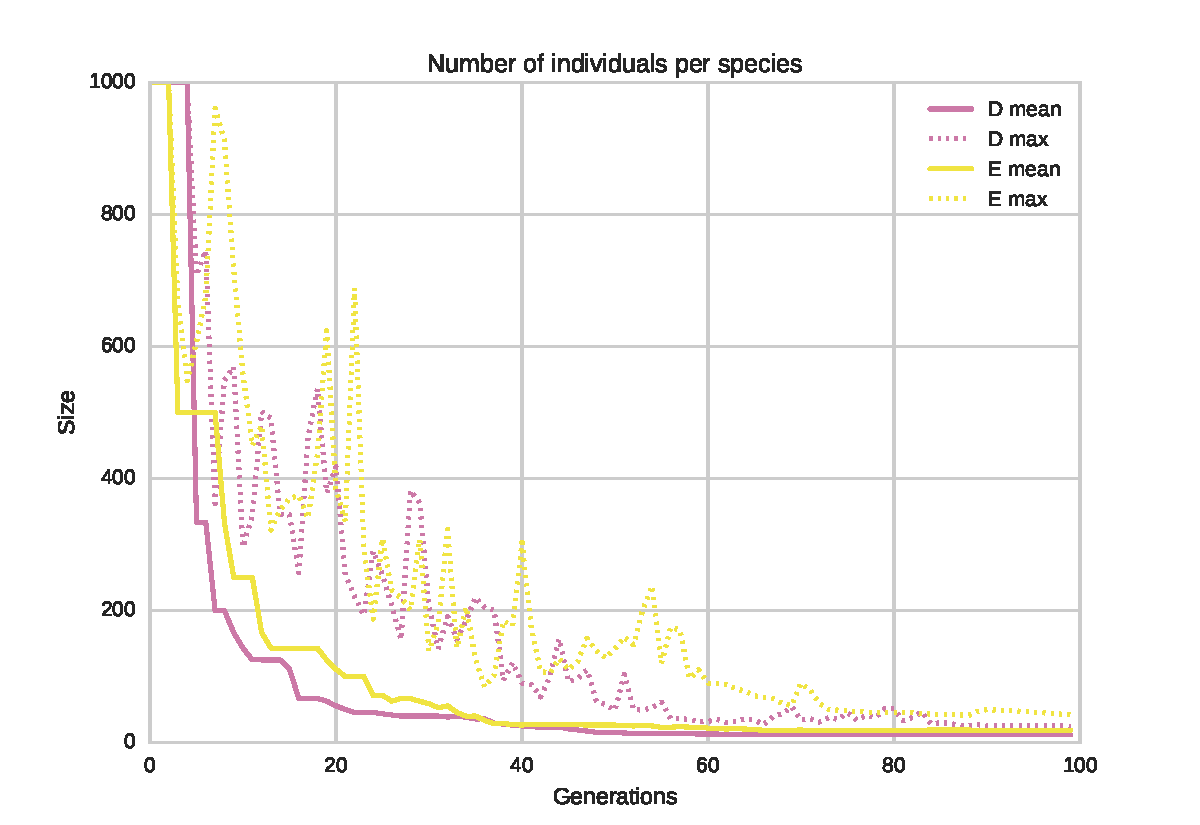
\includegraphics[width=\columnwidth]{fig/species_size}
\caption{The mean and max number of members in the species of scenarios D and E over time}
\label{fig:species_size}
\end{figure}

Another GA property that can be studied is the NEAT-specific speciation in scenarios D and E.
Figure \ref{fig:species} shows the number of different species over time.
Both follow approximately the same development in the first 40 generations, before D overtakes E and they stabilize at different levels.
The difference in levels is quite significant.
A speculative reason for this is that the lack of elitism in D means that a species there is more likely to split into multiple species by chance.
Whereas with elitism in E, the members of the species may be more likely to remain more similar to the elite in the population, leading to less diversity \textit{within} the species.

Figure \ref{fig:species_size} shows the mean number of members per species over time.
The development is as one would expect with the growing number of species seen in Figure \ref{fig:species}, declining more rapidly at first then gradually stabilizing.
The accompanying plot of the max number of species members gives an indication of the variance of the underlying data.
It fluctuates a lot at first, but as 100 generations approach,
the max stabilizes and is only slightly higher than the mean, indicating that the population consists of many species approximately the same (low) number of members.

In the case where there is elitism, as the species size approaches the number of elites ($E=1$) there is less room for innovation in that species, since one member of each species is always a copy of a previous one.
If the size were to reach $1$, there would be no innovation at all happening.
Since the population of scenario E seems to have stabilized around 55 species, a mean species size around $1000 / 55 \approx 18$ should avoid this problem and leave room for innovation.

\subsection{$\lambda$}
\begin{figure}
\centering
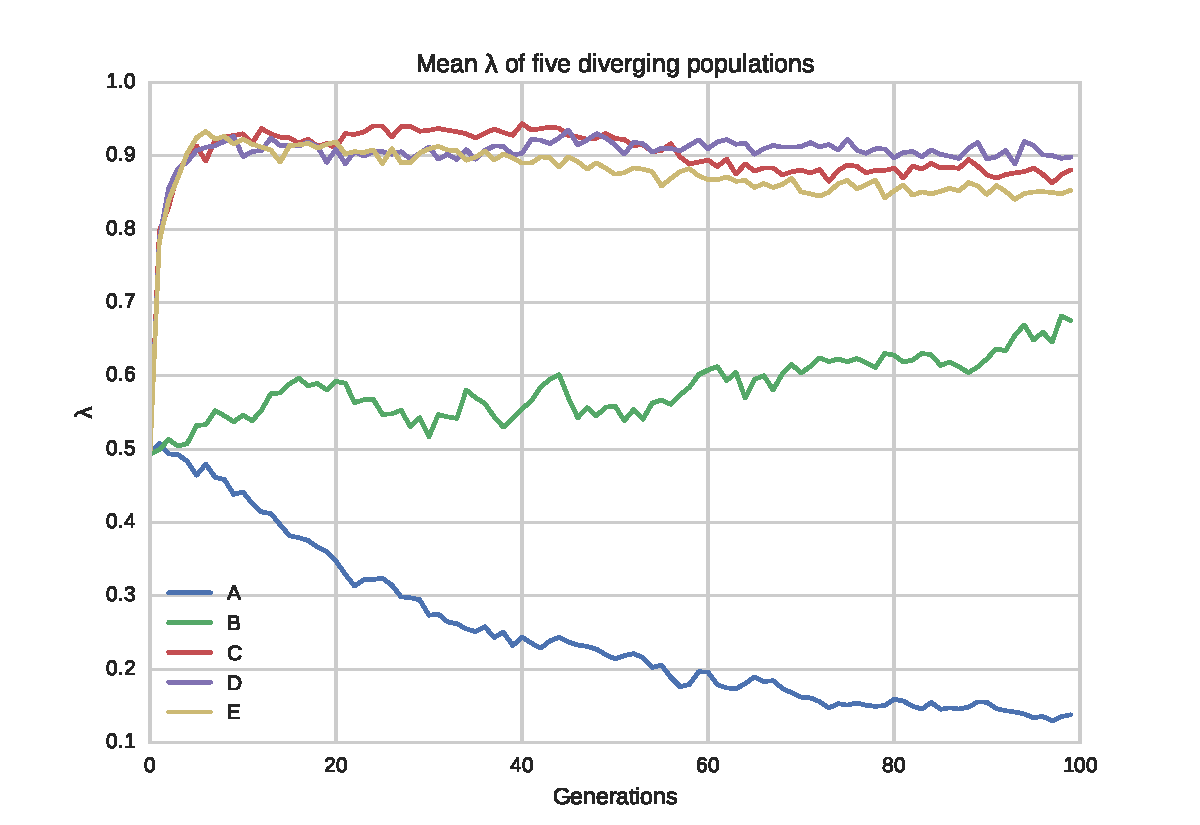
\includegraphics[width=\columnwidth]{fig/mean_lambda}
\caption{Development of the mean $\lambda$ of five scenarios over time}
\label{fig:lambda_over_t}
\end{figure}

\begin{figure}
\centering
\begin{subfigure}[t]{.49\columnwidth}
\centering
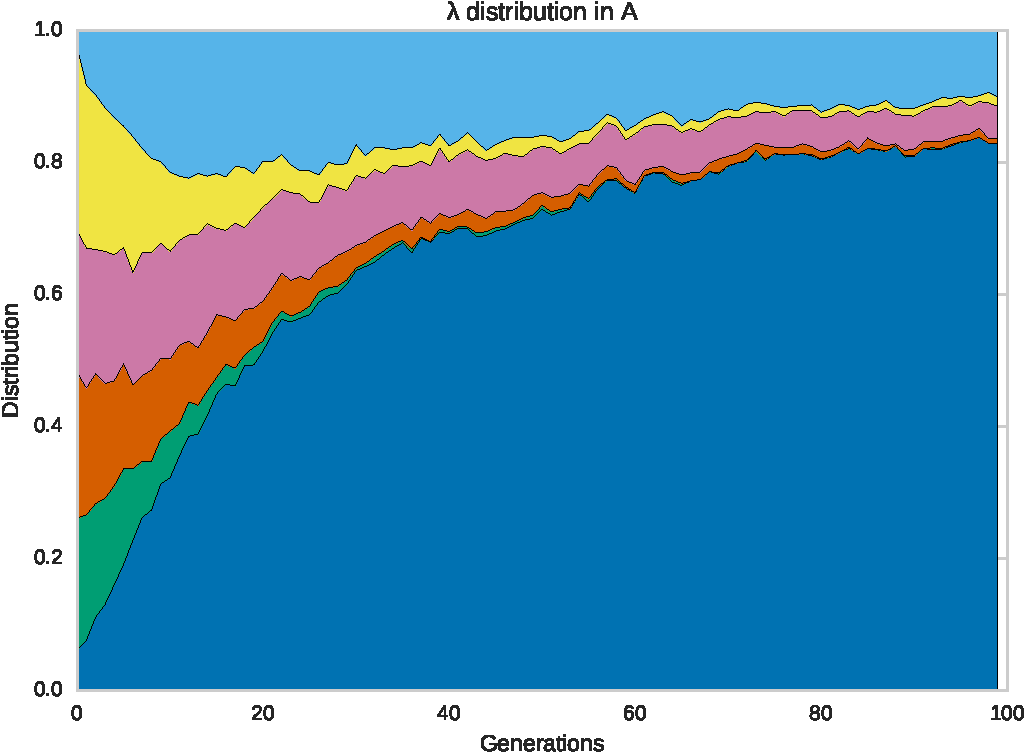
\includegraphics[width=\columnwidth]{fig/lambda_A}
\caption{Scenario A}
\label{fig:lambda_A}
\end{subfigure}
\begin{subfigure}[t]{.49\columnwidth}
\centering
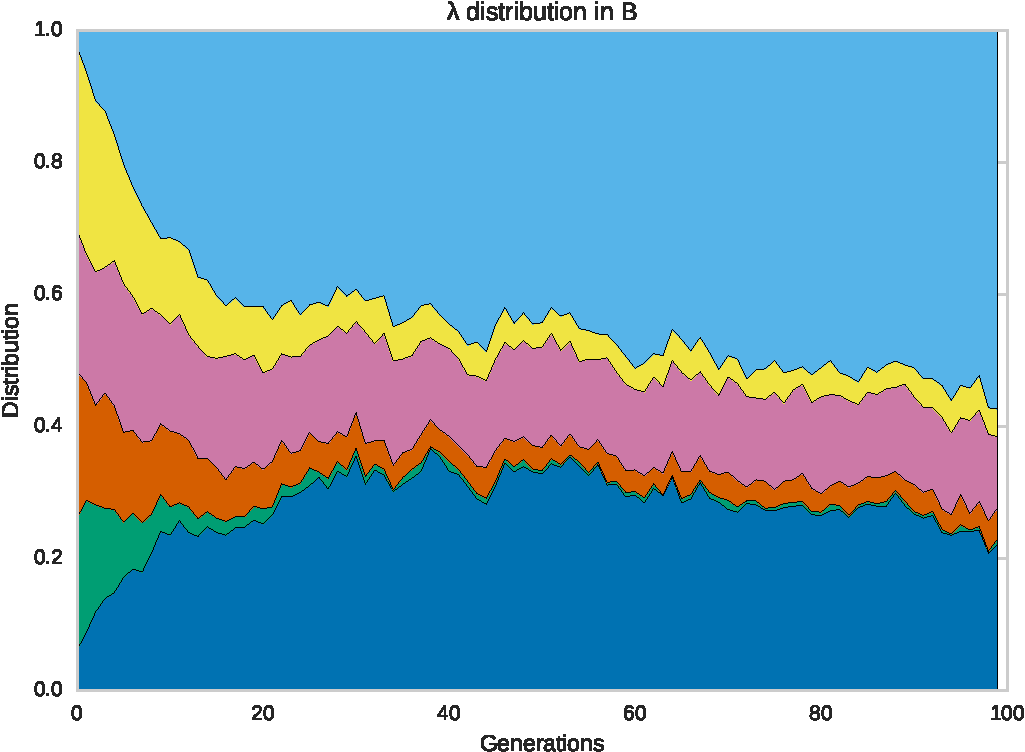
\includegraphics[width=\columnwidth]{fig/lambda_B}
\caption{Scenario B}
\label{fig:lambda_B}
\end{subfigure}
\begin{subfigure}[t]{.49\columnwidth}
\centering
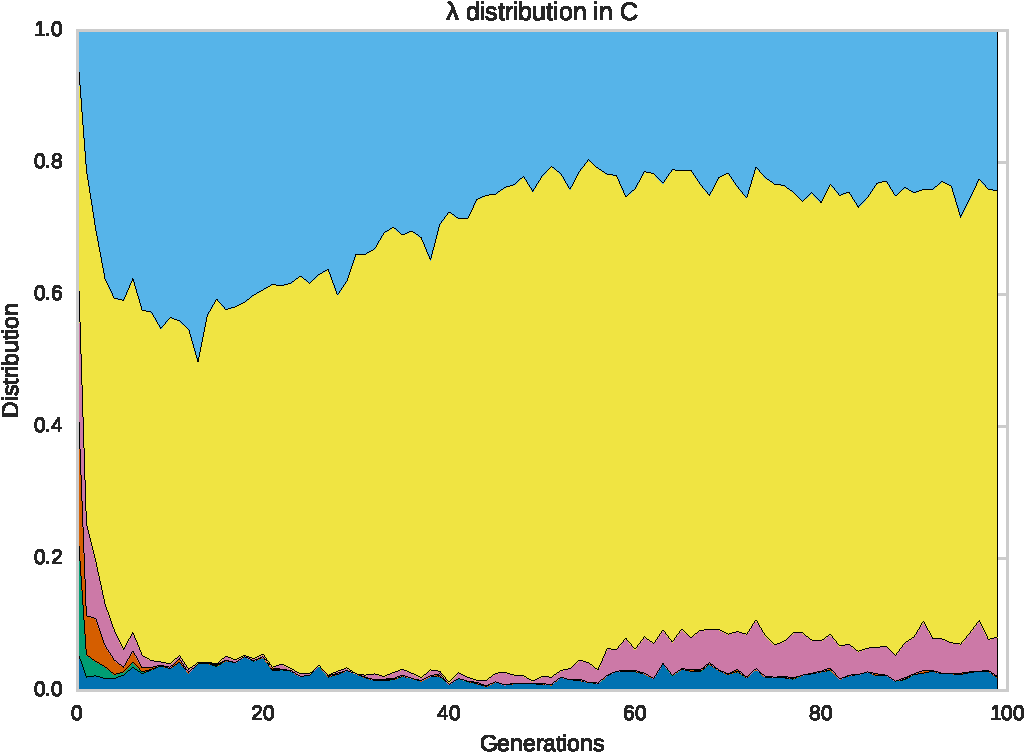
\includegraphics[width=\columnwidth]{fig/lambda_C}
\caption{Scenario C}
\label{fig:lambda_C}
\end{subfigure}
\begin{subfigure}[t]{.49\columnwidth}
\centering
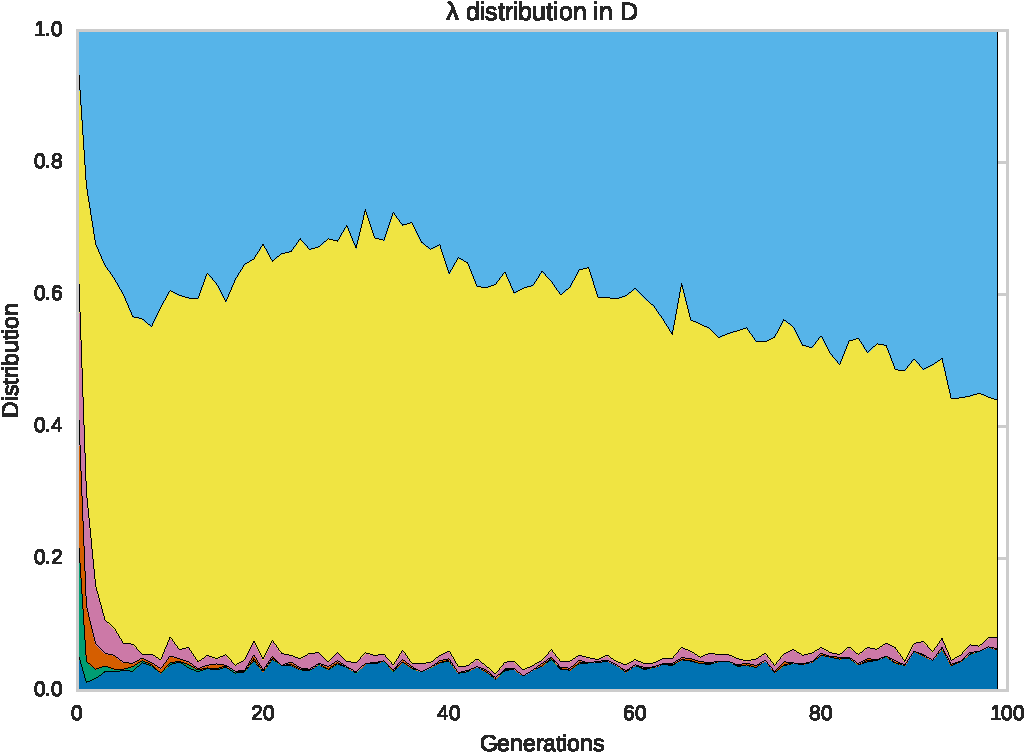
\includegraphics[width=\columnwidth]{fig/lambda_D}
\caption{Scenario D}
\label{fig:lambda_D}
\end{subfigure}
\begin{subfigure}[t]{.49\columnwidth}
\centering
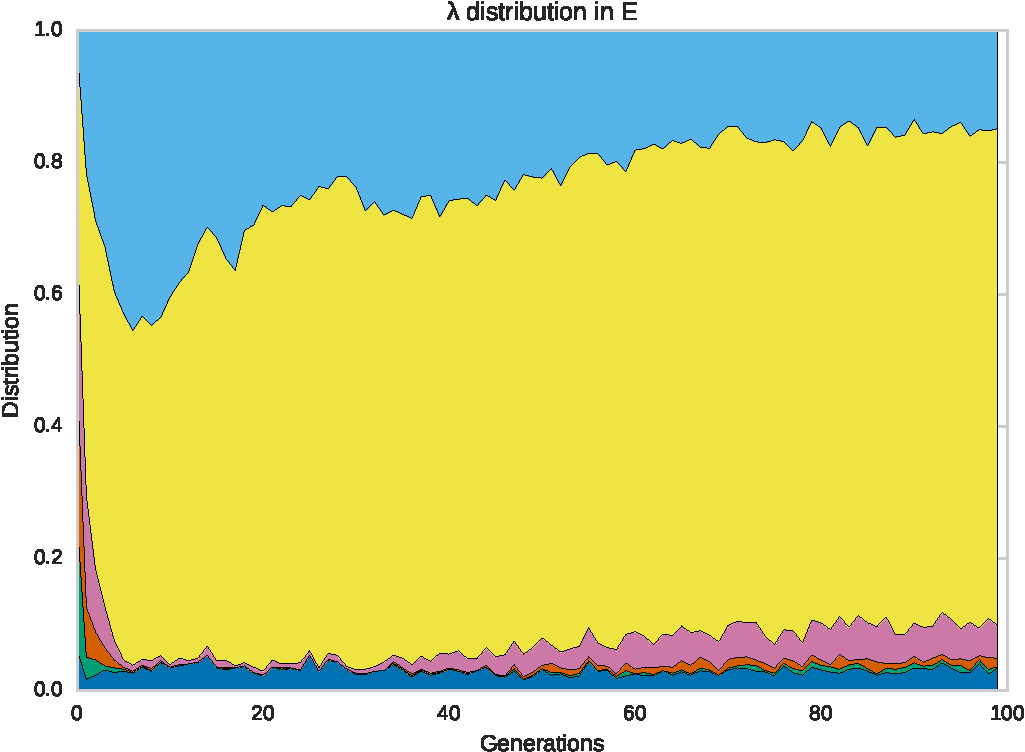
\includegraphics[width=\columnwidth]{fig/lambda_E}
\caption{Scenario E}
\label{fig:lambda_E}
\end{subfigure}
\begin{subfigure}[t]{.49\columnwidth}
\centering
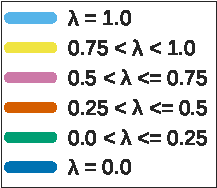
\includegraphics[width=\columnwidth, height=4.5cm, keepaspectratio]{fig/lambda_legend}
\caption{Legend}
\end{subfigure}

\caption{Breakdown of $\lambda$ distribution over time in five scenarios}
\label{fig:lambdas_breakdown}
\end{figure}

The $\lambda$ parameter is an interesting property of a CA transition function to study.
Figure \ref{fig:lambda_over_t} shows the mean $\lambda$ over time for the five scenarios.
The shapes of the curves have a lot of similarities with the shapes of the fitness curves in Figure \ref{fig:f_over_t}.
The random mutation in scenario A drives the mean $\lambda$ towards $0$,
while the combination of mutation and crossover without selection pressure of scenario B causes the $\lambda$ to fluctuate a lot and increase slightly, but not very significantly.
Scenarios C, D and E have roughly the same development: a sharp rise to about $0.9$, then flattening out.
%Both D and E do a slight "correction" afterwards, slowly decreasing after the initial rapid rise.

Figure \ref{fig:lambdas_breakdown} shows the scenarios broken down individually into stack plots, illustrating the distribution of values changing over time.
The values are sorted into six bins, two special ones for $\lambda$ exactly equal to $0.0$ and $1.0$ and four for the equal intervals in between.
In earlier experiments it was observed that the two extreme $\lambda$ occur often, so they get special bins in this visualization.

It can be seen that the scenario A has a very strong bias towards producing $\lambda = 0.0$,
while the other scenarios skew more towards producing higher $\lambda$ values.
This would suggest that crossover mechanism is at least partially responsible for producing higher $\lambda$ values.
There is also a strong resemblance between C and E, less so between D and the others.
Why this is so is not entirely obvious, but it could just be a consequence of the randomness of the trial.
If the experiment was repeated with multiple trials, we could determine if this is just a fluke or not.
In any case, it is clear that all the scenarios with selection pressure are strongly biased towards producing $\lambda > 0.75$.

The task at hand and the implementation of the fitness function must also be considered when analyzing the $\lambda$ result.
The fitness evaluation function is described in detail in Section \ref{sec:morph_problems}.
Notably, when trying to produce a "Swiss flag" pattern, 
$20/25$ cells are active in the target state, meaning that the algorithm can get \textit{some} score easily by producing a transition function with $\lambda = 1.0$.
This can explain why the algorithm produces very many $\lambda=1.0$ solutions early on.
%Considering this, as well as Langton's theory of the "Edge of Chaos", the breakdowns seen in C, D and E make sense.

%\begin{figure}
%\centering
%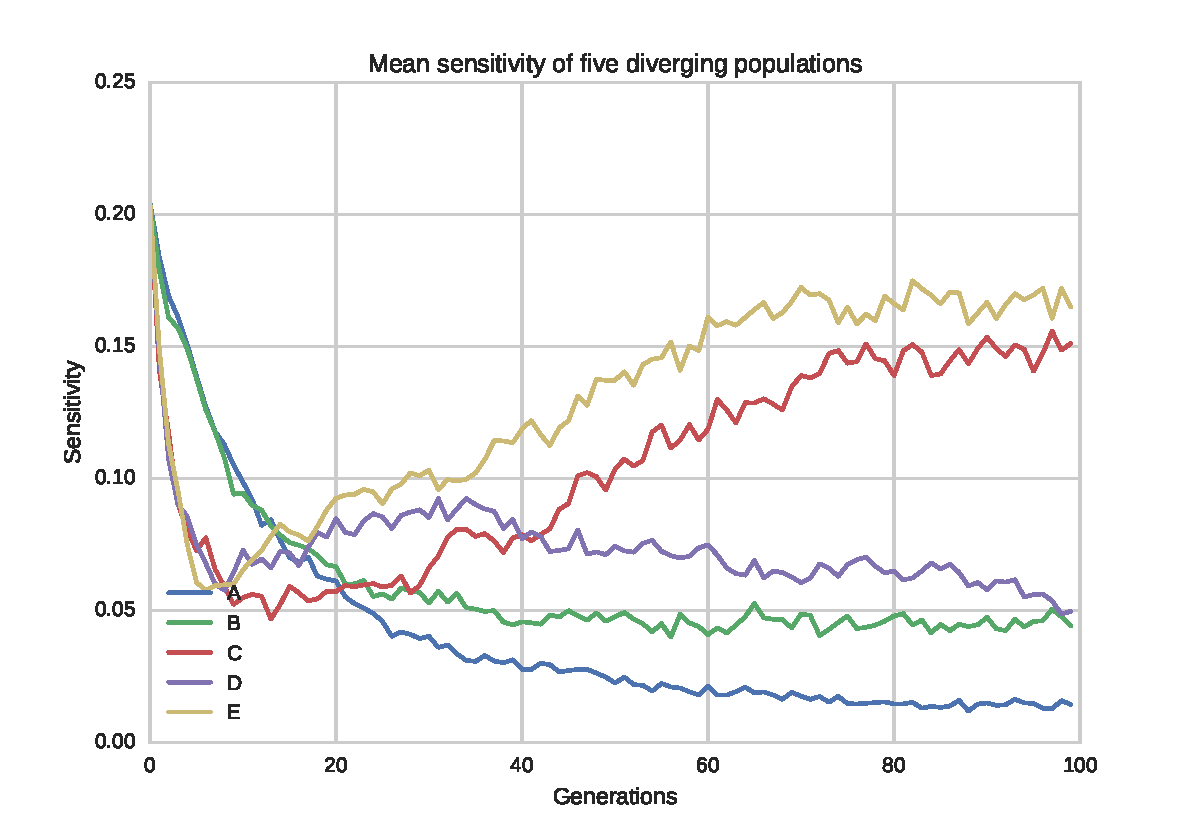
\includegraphics[width=\columnwidth]{fig/sensitivity}
%\caption{TODO}
%\label{fig:sensitivity}
%\end{figure}

%\begin{figure}
%\centering
%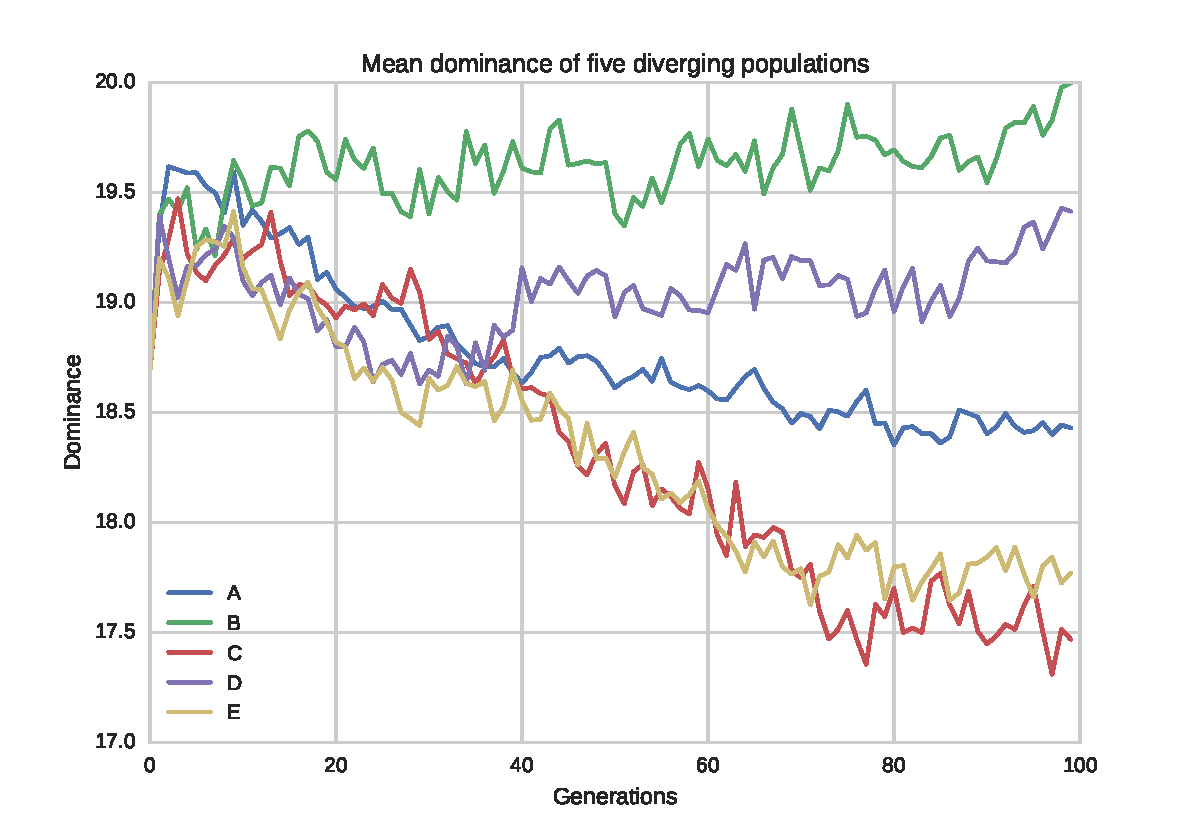
\includegraphics[width=\columnwidth]{fig/dominance}
%\caption{TODO}
%\label{fig:dominance}
%\end{figure}


\subsection{Distinct behaviors}
\begin{figure}
\centering
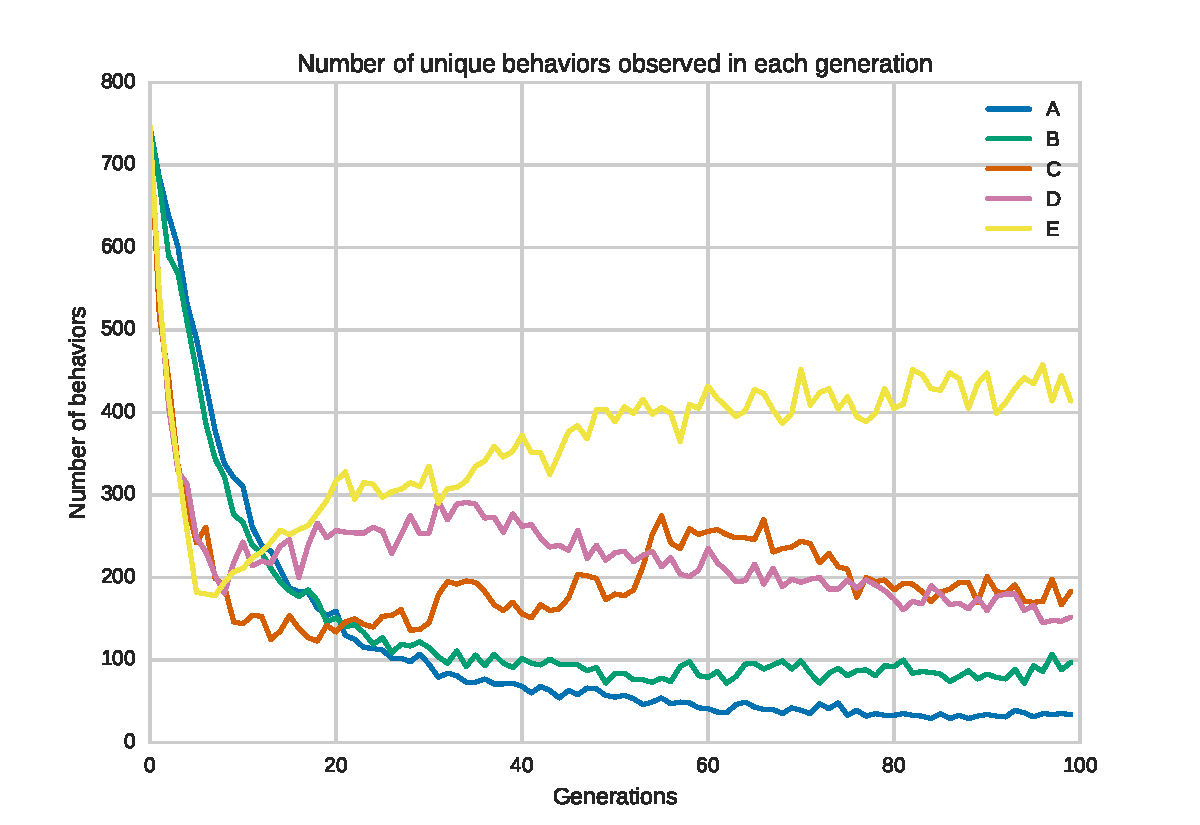
\includegraphics[width=\columnwidth]{fig/unique_behaviors}
\caption{Number of unique behaviors in each generation}
\label{fig:unique_behaviors}
\end{figure}

\begin{figure}
\centering
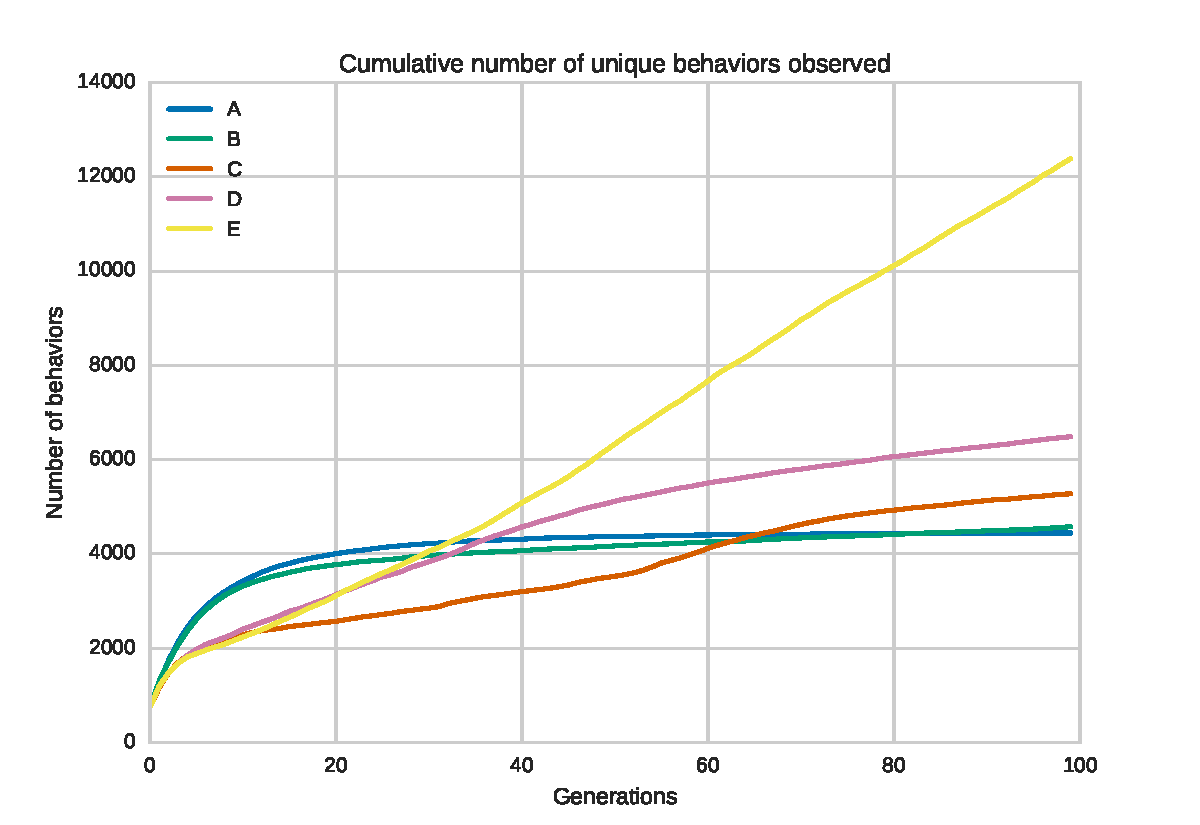
\includegraphics[width=\columnwidth]{fig/cummulative_unique_behaviors}
\caption{
    Number of unique behaviors seen over time, cumulative.
}
\label{fig:cummulative_unique_behaviors}
\end{figure}

\begin{figure}
\centering
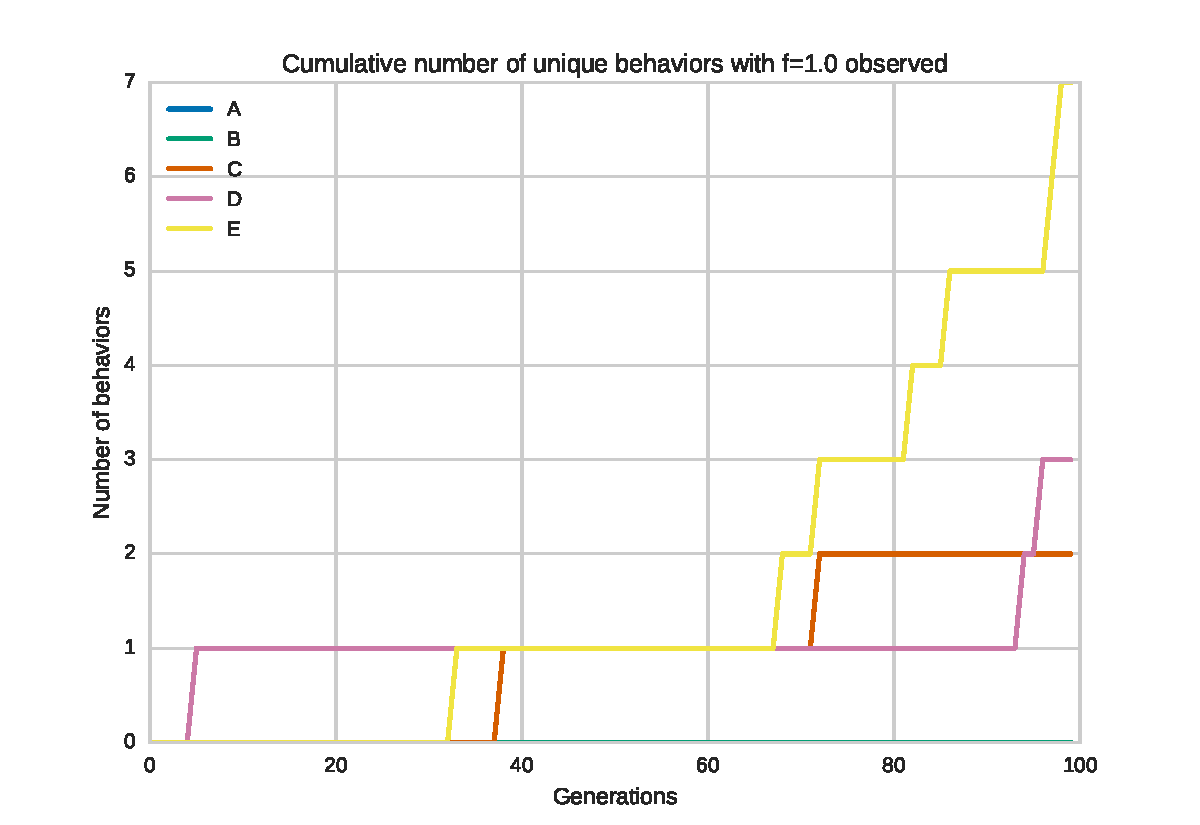
\includegraphics[width=\columnwidth]{fig/cummulative_unique_perfect}
\caption{
    Number of unique $f=1.0$ behaviors seen over time, cumulative.
}
\label{fig:cummulative_unique_perfect}
\end{figure}

%\begin{figure}
%\centering
%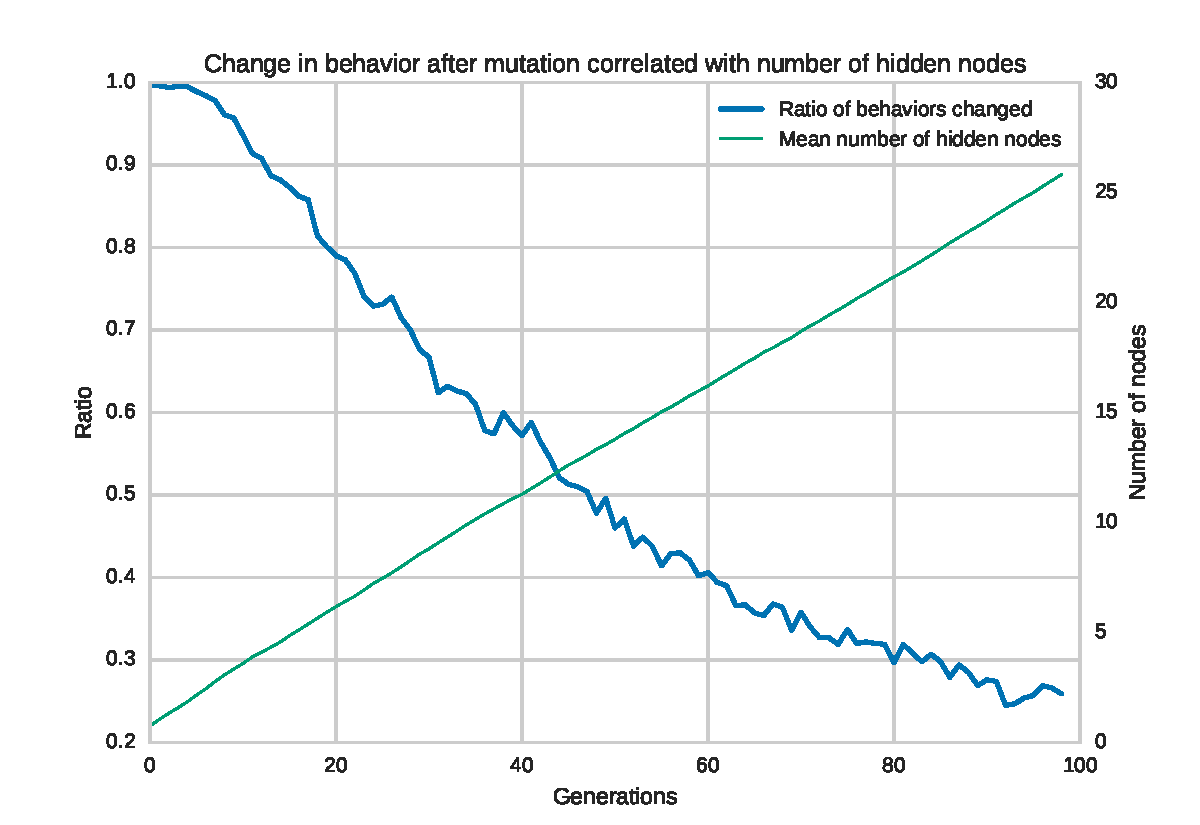
\includegraphics[width=\columnwidth]{fig/mutation_behavior_change}
%\caption{Ratio of genotypes that change behavior after mutation}
%\label{fig:mutation_behavior_change}
%\end{figure}

%Studying the $\lambda$ parameter can give some insights, but it does not capture every aspect of the transition function behavior.
Another way to analyze the population is to look at the diversity of the enumerated behavior "strings" over time.
Figure \ref{fig:unique_behaviors} shows how many unique behaviors are present in each generation of each scenario.
The initial population is clearly very diverse, but the diversity drops very rapidly in each of the scenarios.
Scenarios A and B decrease slightly slower than the rest at the beginning.
The rate of decreasing slows down and they eventually stabilize at low levels.
Scenarios C, D and E drop down fast at first, but then they do a sharp turn.
C and D fluctuate a it up and down, but overall seem to stabilize.
E rises steadily again and stabilizes at a significantly higher level than the others.

Figure \ref{fig:cummulative_unique_behaviors} visualizes the number of unique behaviors seen in the entire lifetime of the scenario.
A and B are almost identical, showing almost no increase after the first 20 generations.
C and D climb steadily and overtake A and B at different points.
The contrast between E and the rest is stark.
There is a much higher rate of increase, and it is almost linear over time, reaching about twice the value that the next best does in 100 generations.
These result have some big implications.
First of all, it is clear that a random search such as A and B gets "stuck" quite quickly and stops producing innovative results.
With selection pressure, the search is slower at first, needing quite some time to overtake the initial flood of innovation produced by randomness.
But it keeps a steady increase where the random search stops.
And the presence of elitism increases the innovation by a very considerable degree.

In a "best-case" where every behavior in every generation is distinct,
the number of unique behaviors observed would be $P * G = 100000$.
Scenario E passes 12000 unique behaviors observed, which is "only" 12\% of the theoretical maximum.
And for a $K=2, N=5$ CA, the number of total possible behaviors is $K^{K^N} = 2^{32} \approx 4.3 * 10^9$.
This illustrates the futility of attempting to solve advanced CA tasks by exhaustive enumeration of behaviors.
Luckily, while the proverbial haystack may be humongous,
there are many needles to be found within it, and you only need to find one to be successful.
Figure \ref{fig:cummulative_unique_perfect} illustrates the number of distinct behaviors observed with a perfect fitness score.
As one might expect, the diversity of the optimal behaviors is higher when the diversity of all behaviors is higher.
Scenario E is able to find 7 distinct solutions to the task.

\subsection{Network Topology}
\begin{figure}
\centering
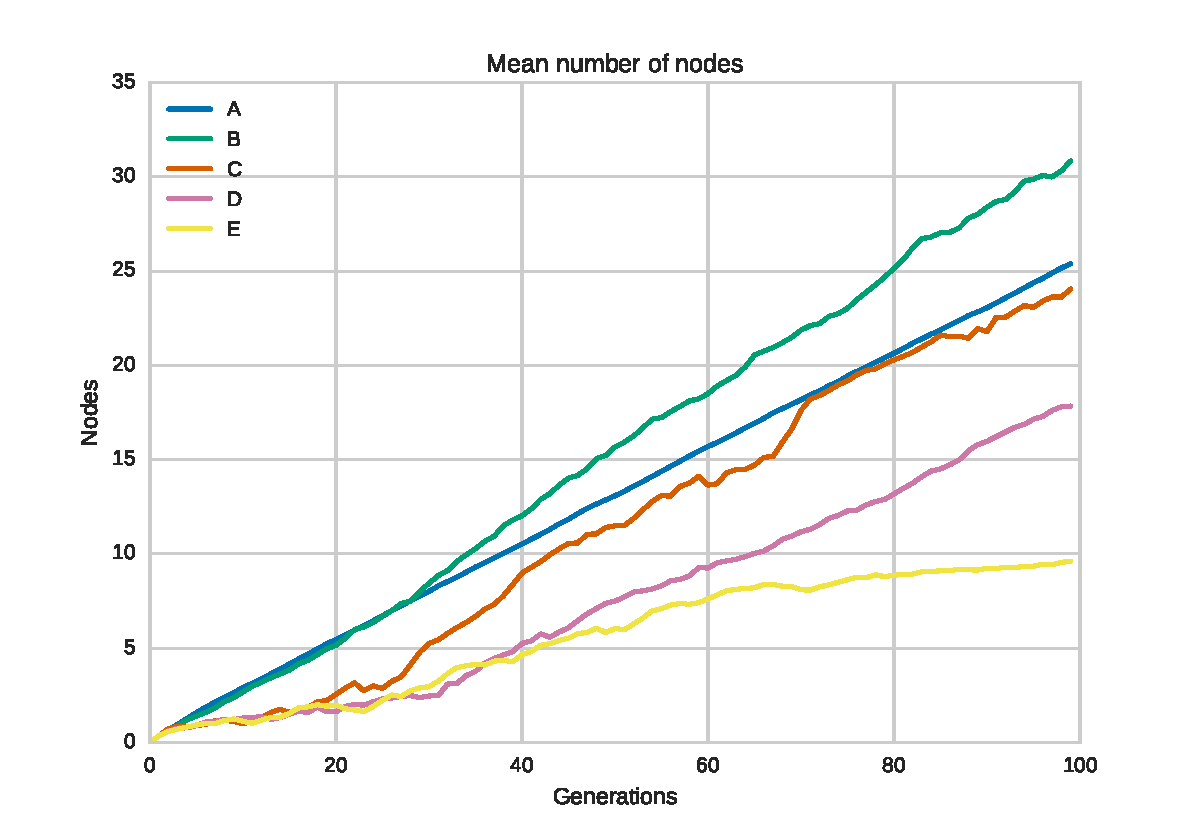
\includegraphics[width=\columnwidth]{fig/sizes}
\caption{The mean number of nodes in each scenario}
\label{fig:sizes}
\end{figure}

\begin{figure}
\centering
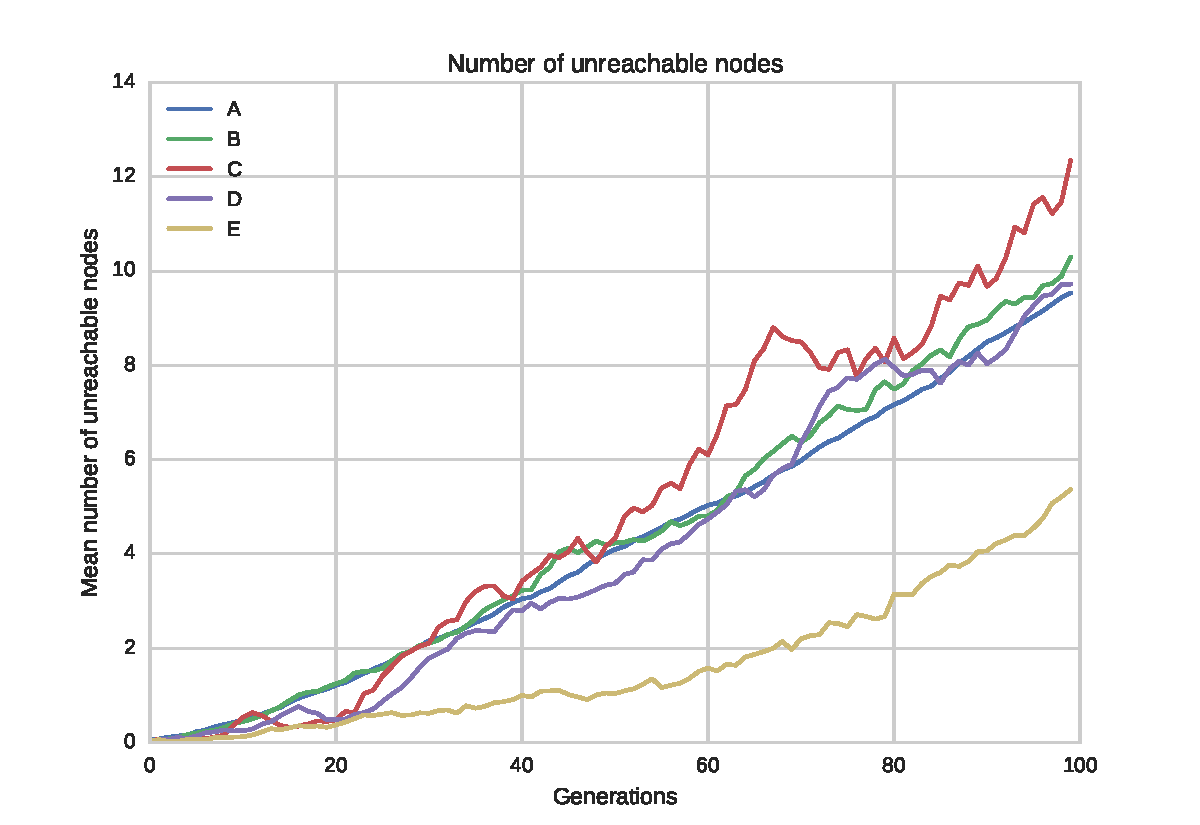
\includegraphics[width=\columnwidth]{fig/vestigial_nodes}
\caption{The mean number of disconnected nodes in each scenario}
\label{fig:vestigial_nodes}
\end{figure}

%\begin{figure}
%\centering
%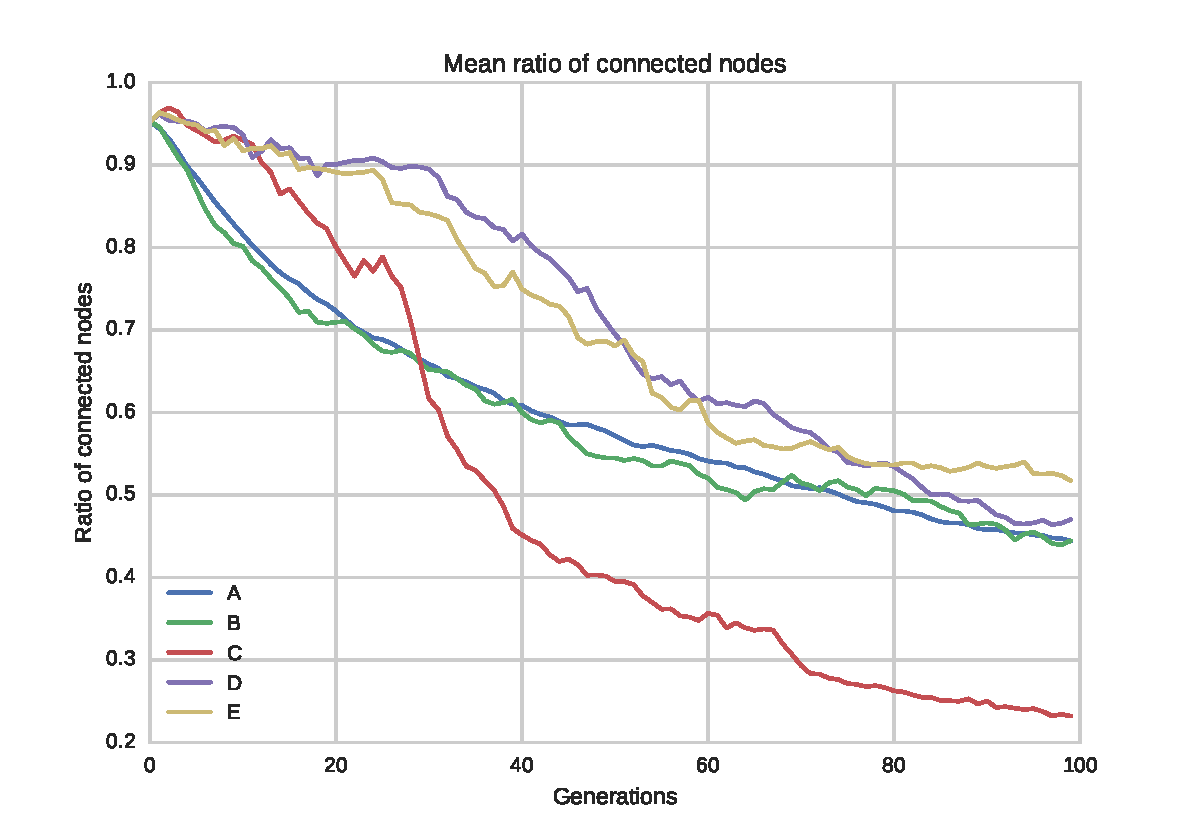
\includegraphics[width=\columnwidth]{fig/vestigial_ratio}
%\caption{The ratio of connected nodes in each scenario}
%\label{fig:vestigial_ratio}
%\end{figure}

\begin{figure}
\centering
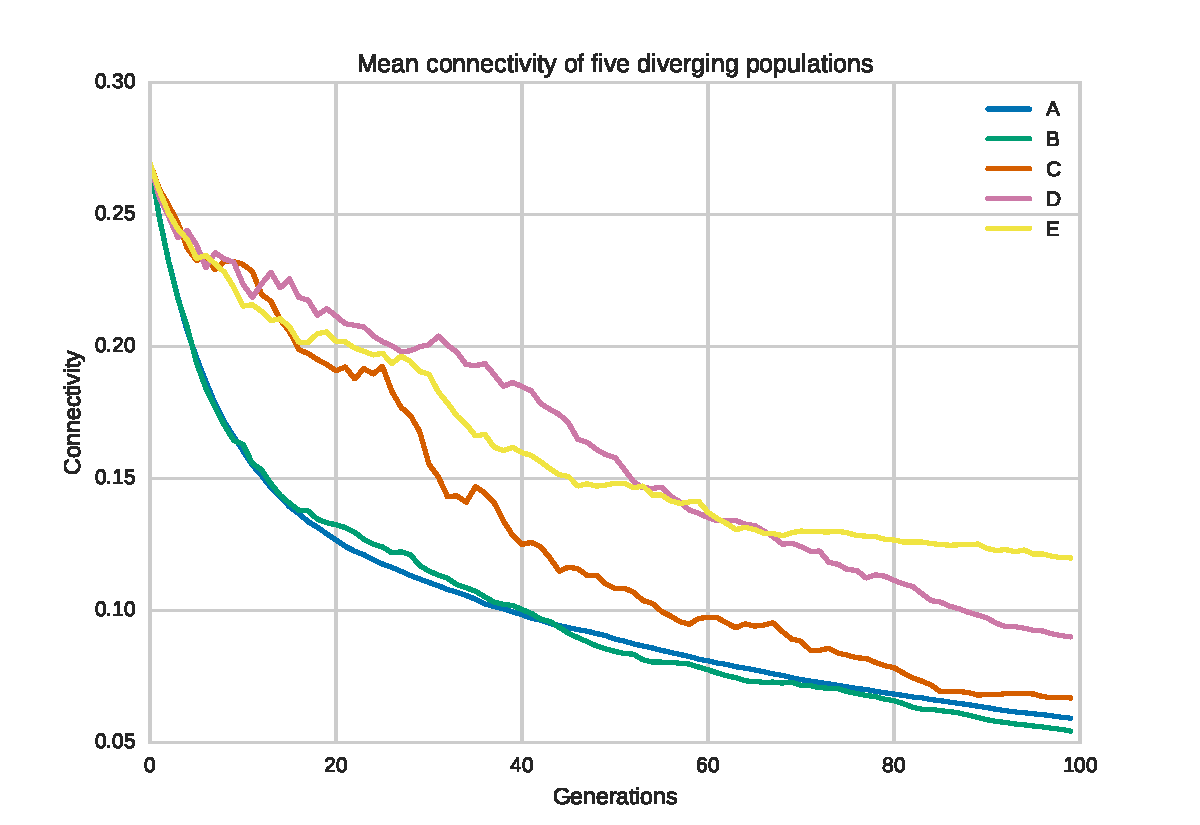
\includegraphics[width=\columnwidth]{fig/connectivity}
\caption{The mean connectivity degree in each population}
\label{fig:connectivity}
\end{figure}

The individuals of the populations are graph structures, and can also be studied as such.
Figure \ref{fig:sizes} shows the development of the mean number of nodes in the networks of each scenario.
The growth of scenario A is approximately linear.
Since the individuals of the population are completely independent from each other,
the law of large numbers means that the curve should fit the expected value given by the probabilities of adding and removing nodes, $(P_\text{add} - P_\text{remove})x = (0.5 - 0.25)x = 0.25x$.
This is not a very useful insight by itself, but it does give a baseline which the other scenarios can be compared to.
Scenario B has a slightly higher growth than A.
This makes sense considering the crossover mechanism.
If two parents independently are likely to gain a new node, then their child will have both of the new nodes, leading to a bigger growth rate overall.
The three scenarios with selection pressure at first follow the same pattern, with much lower growth than the baseline.
Then they diverge around 30 generations.
Scenario C "catches up" with scenario A and settles into a near-linear growth like scenario A.
Scenario D also goes into a linear growth close to the same as scenario A, but without "catching up" first.
Scenario E continues with almost the same growth rate for all 100 generations, ending up at a much lower number than the rest.

Figure \ref{fig:vestigial_nodes} shows the number of "vestigial" nodes that do not connect to the output layer.
The significance of these is that they are equally likely to be affected by mutation as any other node, but they do not affect the output of the network.
The more vestigial nodes there are, the more likely that the mutation operation does "nothing".

Scenarios A and B have curve shapes very similar to those they had in Figure \ref{fig:sizes}, suggesting a simple proportional correlation when the process is completely random.
More interestingly, the curve of scenario C does a sudden turn to overtake both A and B.
The curve of C reaches almost the same value as that in Figure \ref{fig:sizes}, indicating the population members have a very large number of disconnected nodes.
The curves of D and E are similar to their counterparts in Figure \ref{fig:sizes}.
Again it is clear that E has a distinctly different development than the rest.

%Figure \ref{fig:vestigial_ratio} shows the relationship between Figures \ref{fig:sizes} and \ref{fig:vestigial_nodes}.
%Scenarios A and B run a very parallel course here, as does D and E.
%The four actually end up near the same value at 100 generations.
%C on the other hand, goes off to do its own thing completely here, and as noted earlier, ends up at a very low ratio of connectedness.

Figure \ref{fig:connectivity} shows another measure of connectedness which is often used in graph theory, $\text{connectivity} = \frac{c}{\sum_{x=1}^{n}{x}}$, where $c$ is the number of connections and $n$ is the number of nodes.
In this perspective, C follows D and E at first, but diverges and drops much quicker to the level of A and B.

What these observations seem to indicate, is that the population of C comes to be dominated by networks with many nodes and fewer connections.
It is likely that in repeated trial this would not occur every time, but that it is just part of the randomness of the single trial.
This is perhaps more likely to occur with the scenario C parameters than the others.
Scenarios A and B are somewhat predictable systems with behavior determined by the constant parameters set before the experiment.
The selection pressure of C can possibly act as a feedback loop, causing a random feature to dominate the whole population.
Scenarios D and E have speciation which automatically create (somewhat) independent trials within the population.

TODO round off this section with some overarching general discussion, maybe in the next chapter
